\documentclass[final]{beamer}
\usetheme{RJH}
\usepackage[orientation=portrait,size=a0,scale=2,debug]{beamerposter}
\usepackage[absolute,overlay]{textpos}
\setlength{\TPHorizModule}{1cm}
\setlength{\TPVertModule}{1cm}

\usepackage[style=science,maxnames=2]{biblatex}
\bibliography{poster}
\def\bibfont{\scriptsize}
\defbibheading{none}{}

\DeclareBibliographyCategory{refs}

% Count total number of entries in each refsection
\AtDataInput{%
  \csnumgdef{entrycount:\therefsection}{%
    \csuse{entrycount:\therefsection}+1}}

% Print the labelnumber as the total number of entries in the
% current refsection, minus the actual labelnumber, plus one
\DeclareFieldFormat{labelnumber}{\mkbibdesc{#1}}    
\newrobustcmd*{\mkbibdesc}[1]{%
  %\number\numexpr\csuse{entrycount:\therefsection}+1-#1\relax}
  \number\numexpr#1\relax}

\title{Mapping antigenic variation in HIV-1 envelope}
\author{\textbf{Simon DW Frost}, University of Cambridge}
\footer{Funded by the Medical Research Council and the Royal Society. Contact: Dr. Simon Frost (\texttt{sdf22@cam.ac.uk})}
\date{}

\begin{document}
\nocite{*}
\setlength{\bibitemsep}{4pt plus 2pt}
\setlength{\bibhang}{20pt}
\addtocategory{refs}{Georgiev2013a,Oh2001,Ping2013,vanGils2010,Kirchherr2011}

\begin{frame}{} 

% Define columns here

\begin{textblock}{9}(1.5,0.3)
\includegraphics[width=5cm]{uc-arms.pdf}
\end{textblock}

\begin{textblock}{6}(77,0.4)
\includegraphics[width=5cm]{image_normal.jpg}
\end{textblock}

\begin{textblock}{40}(1,6.5)
\begin{block}{Background}
\begin{itemize}
\item{Recombinant-virus based assays of neutralisation of HIV-1 envelope are routinely used to measure the sensitivity of viruses to neutralisation, and the ability of sera to neutralise viral isolates.}
\item{It is difficult to visualise antigenic differences, especially when the number of viruses and sera are large.}
\item{\textbf{I present a statistical model to map viruses and sera into antigenic space, and apply it to data from five published studies of HIV-1 neutralisation.}}
\end{itemize}
\end{block}

\begin{block}{Materials and Methods}
\begin{itemize}
\item{Data on neutralisation were from published studies were analysed using Bayesian unfolding multidimensional scaling:}
\begin{itemize}
\item{The model estimates $X$, a $n$ by $p$ matrix of coordinates in antigenic space of viruses, and  $Y$, a $k$ by $p$ matrix of coordinates in antigenic space of plasma samples.}
\item{Let $y_{ij}$ denote the ${\rm log}_2$ transformed ${\rm IC}_{50}$ neutralization titer between virus $i$ and plasma $j$}
\item{The observed dissimilarity measure, $d_{ij}$, was obtained by normalizing the data using the maximum neutralization for each titer, $d_{ij}=\max y_{i \cdot} - y_{ij}$}
\item{$d_{ij}$ is assumed to follow a truncated normal distribution, $d_{ij}\sim N (\delta_{ij}, \tau),\;I(d_{ij}>0)$, where $i=1, \ldots ,n,\;j=1,\ldots,k$}
\item{$\delta_{ij}$ was calculated assuming a two dimensional map.}
\end{itemize}
\end{itemize}
\end{block}

\begin{block}{Analysis of Kirchherr et al. (2011)}
\begin{tabular}{ll}
{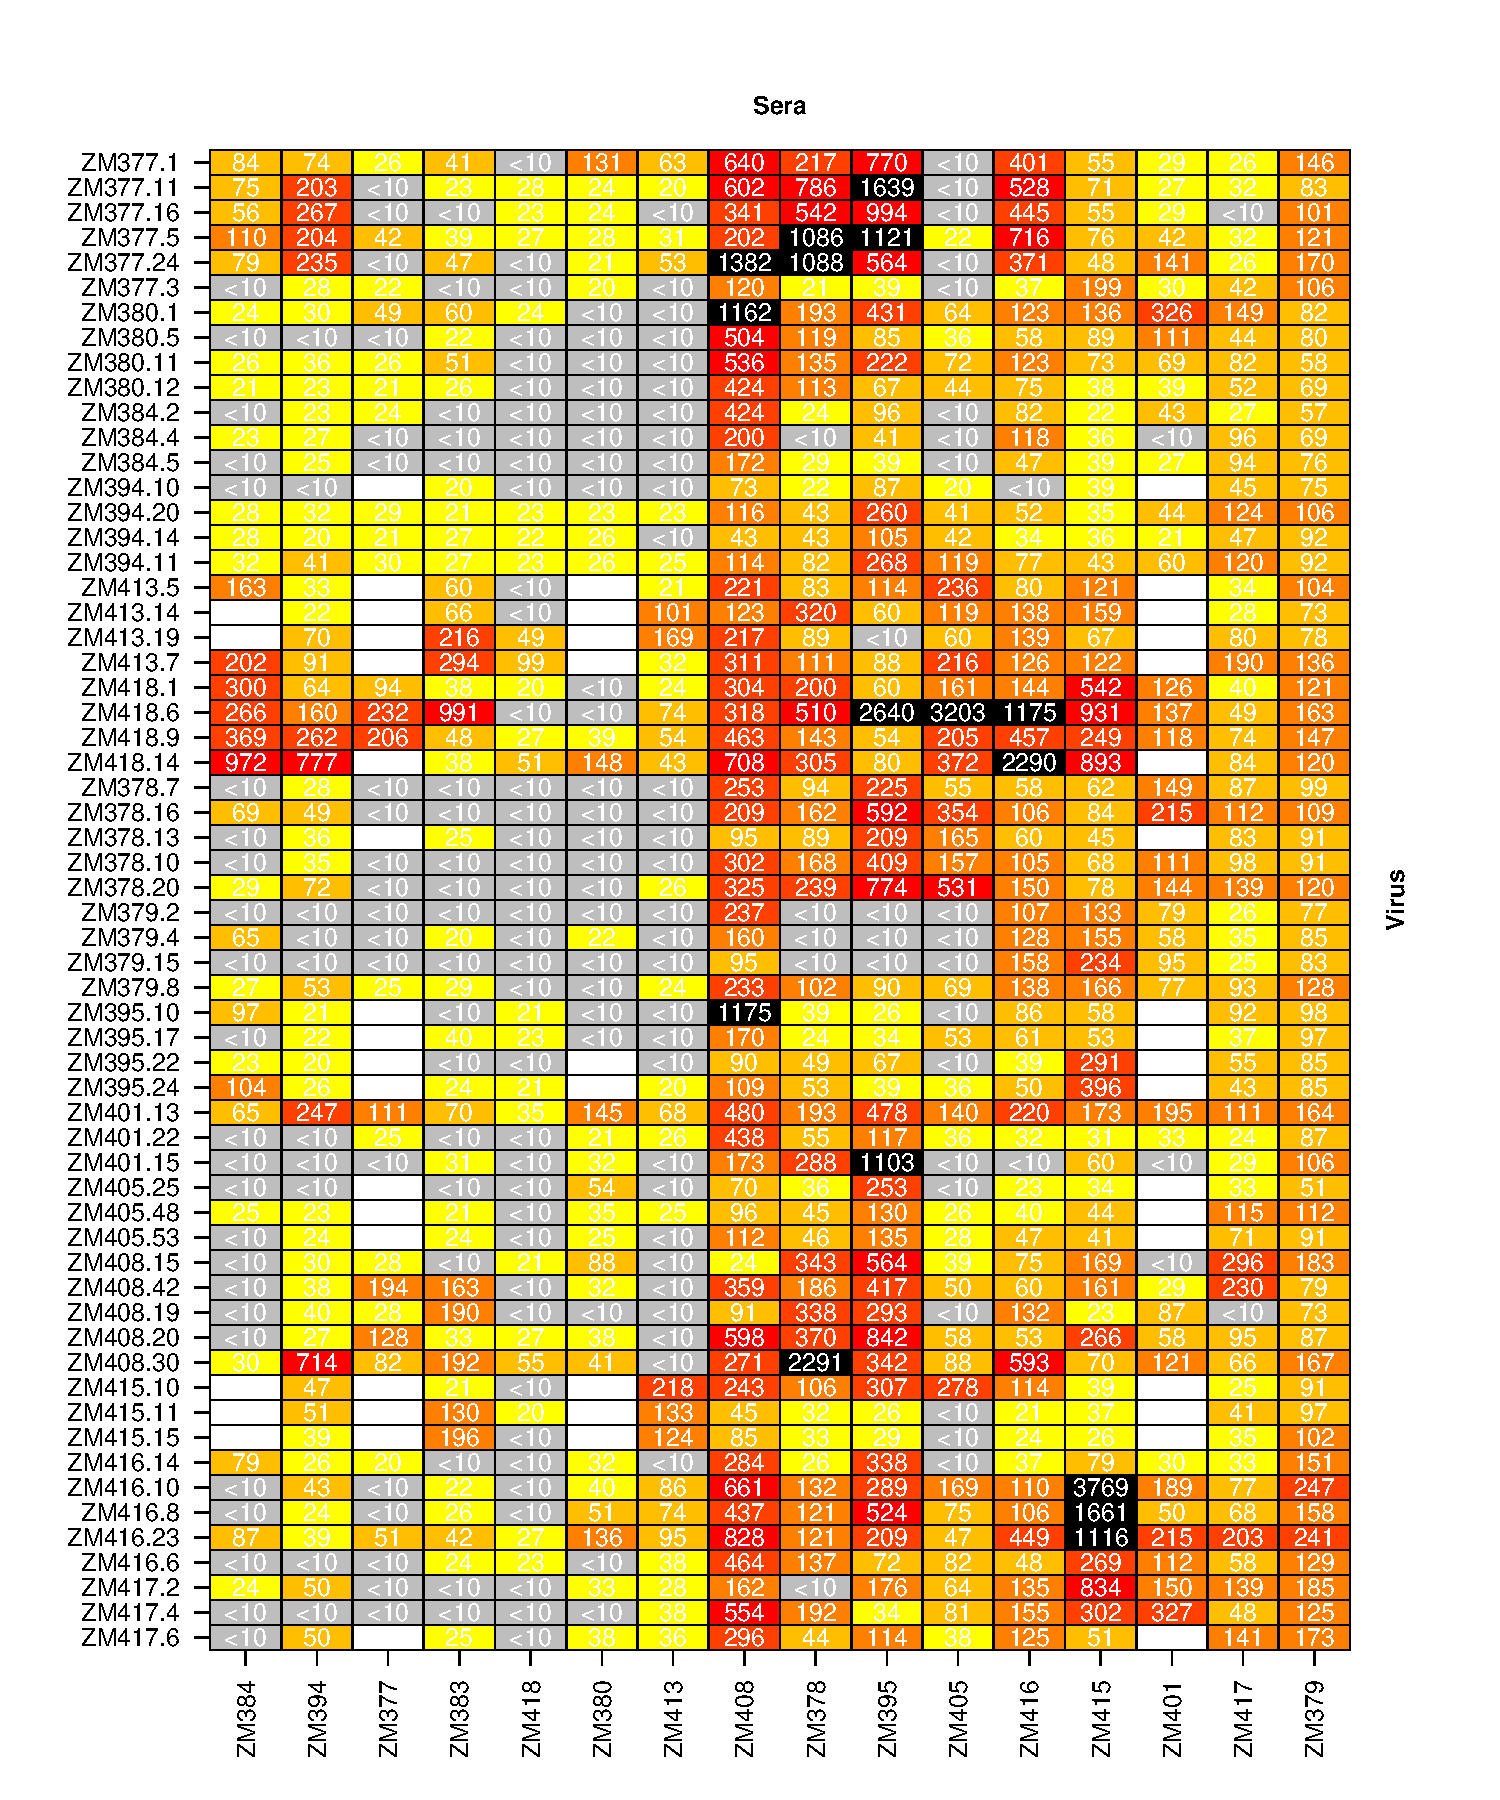
\includegraphics[width=19.5cm]{kircherrtable.pdf}} & \raisebox{11cm}{\parbox{18cm}{
60 viruses (including multiple isolates from the same patients), 16 sera
\begin{itemize}
\item{Hard to see patterns in the data}
\item{Missing data}
\item{Measurements below the limit of detection}
\end{itemize}
}}
\end{tabular}

\includegraphics[height=8cm]{kircherrmap.pdf}
\begin{itemize}
\item{Interpretation of antigenic map}
\begin{itemize}
\item{Each large square represents a 2-fold difference in neutralisation}
\item{Distance between viruses represents similarity in neutralisation sensitivity}
\item{Distance between sera represents similarity in their ability to neutralise diverse viruses (controlling for magnitude)}
\item{Distances between viruses and sera represent similarity in sensitivity to specific sera, relative to the most sensitive virus in the panel}
\end{itemize}
\end{itemize}
\end{block}

\end{textblock}

\begin{textblock}{40}(43,6.5)

%\begin{block}{Kircherr et al.}
%\begin{itemize}
%\item{60 viruses (including multiple from same patients), 16 sera}
%\end{itemize}
%\includegraphics[height=8cm]{kircherrmap.pdf}
%\end{block}

%\begin{block}{Doria-Rose et al. (2010)}
%\begin{itemize}
%\item{Fix for noncens}
%\end{itemize}
%\includegraphics[height=8cm]{doriamap.pdf}
%\end{block}

\begin{block}{Van Gils et al. (2010)}
\begin{itemize}
\item{23 viruses, subtypes A-D, 15 subtype B sera}
\item{Some apparent clusters of viruses, but \textit{not} related to subtype}
\end{itemize}
\begin{center}
\includegraphics[height=8cm]{vangilsmap.pdf}
\end{center}
\end{block}

\begin{block}{Georgiev et al. (2013)}
\begin{itemize}
\item{21 viruses, 22 sera}
\item{Some clustering of viruses, less antigenic variation than Van Gils et al. (2010)}
\end{itemize}
\begin{center}
\includegraphics[height=8cm]{georgievmap.pdf}
\end{center}
\end{block}

\begin{block}{Ping et al. (2013)}
\begin{tabular}{ll}
{\includegraphics[height=17.5cm]{pingmap.pdf}} & \raisebox{9cm}{\parbox{25cm}{
\begin{itemize}
\item{65 viruses, 9 sera (including two immunoglobulin pools)}
\item{Higher resolution than other datasets; significant two-dimensional variation in the map}
\end{itemize}
}}
\end{tabular}
\end{block}

\begin{block}{Conclusions}
\begin{itemize}
\item{Differences in neutralisation of HIV-1 can be mapped into 1-2 dimensions without significant loss of information}
\begin{itemize}
\item{This approach removes confounding of breadth by the overall magnitude of the response}
 \item{Without knowing the number of antibodies in a sample, we cannot compare sera without normalisation}
 \end{itemize}
 \item{'Broadly-reactive' sera exhibit similar patterns of neutralisation across viral isolates.}
 \item{Extensive, often continuous, antigenic distances between viruses.}
 \begin{itemize}
 \item{Not related to subtype, and only weakly associated with specific positions.}
 \end{itemize}
%\item{\textbf{Antigenic distances were associated with amino acid substitutions across many sites scattered over the whole envelope region}}
%\begin{itemize}
%\item{Antigenic differences between viruses arise due to multiple mutations of relatively small effect.}
%\end{itemize}
\end{itemize}
\end{block}


\begin{block}{References}
\printbibliography[category=refs,heading=none]
\end{block}

\end{textblock}

\end{frame}
\end{document}
